%\documentclass{beamer} 
\documentclass[handout]{beamer} % sin pausas
\usetheme{CambridgeUS}

\usepackage[utf8]{inputenc}%esto permite (en Windows) escribir directamente 
\usepackage{graphicx}
\usepackage{array}
\usepackage{tikz} 
\usetikzlibrary{shapes,arrows,babel,decorations.pathreplacing}
\usepackage{verbatim} 
\usepackage{xcolor} 
\usepackage{amsgen,amsmath,amstext,amsbsy,amsopn,amsfonts,amssymb}
\usepackage{amsthm}
\usepackage{tikz}
\usepackage{tkz-graph}
\usepackage{mathtools}
\usepackage[customcolors]{hf-tikz}


%\setbeamertemplate{background}[grid][step=8 ]
\setbeamertemplate{itemize item}{$\circ$}
\setbeamertemplate{enumerate items}[default]

\definecolor{links}{HTML}{2A1B81}
\hypersetup{colorlinks,linkcolor=,urlcolor=links}

\newcommand{\img}{\operatorname{Im}}
\newcommand{\nuc}{\operatorname{Nu}}
\newcommand\im{\operatorname{Im}}
\renewcommand\nu{\operatorname{Nu}}
\newcommand{\la}{\langle}
\newcommand{\ra}{\rangle}
\renewcommand{\t}{{\operatorname{t}}}
\renewcommand{\sin}{{\,\operatorname{sen}}}
\newcommand{\Q}{\mathbb Q}
\newcommand{\R}{\mathbb R}
\newcommand{\C}{\mathbb C}
\newcommand{\K}{\mathbb K}
\newcommand{\F}{\mathbb F}
\newcommand{\Z}{\mathbb Z}

\renewcommand{\figurename }{Figura}
%\usepackage{enumitem}
%\setlist[itemize]{itemsep=10pt, label={$\circ$}}
%\newtheorem{teorema}{Teorema}
%\newtheorem{corolario}[teorema]{Corolario}
%\newtheorem{proposicion}[teorema]{Proposición}

%\theoremstyle{definition}
%\newtheorem{definicion}[theorem]{Definici\'on}
%\newtheorem{ejemplo}[theorem]{Ejemplo}
%\newtheorem{pregunta}[equation]{Pregunta}
%\newtheorem{step}{Paso}



\newenvironment{exercise}[1]% environment name
{% begin code
	\par\vspace{\baselineskip}\noindent
	\textbf{Ejercicio (#1)}\begin{itshape}%
		\par\vspace{\baselineskip}\noindent\ignorespaces
	}%
	{% end code
	\end{itshape}\ignorespacesafterend
}


\newenvironment{definicion}% environment name
{% begin code
	\par\vskip .2cm%
	{\color{blue}Definición}%
	\vskip .2cm
}%
{%
	\vskip .2cm}% end code

\newenvironment{observacion}% environment name
{% begin code
	\par\vskip .2cm%
	{\color{blue}Observación}%
	\vskip .2cm
}%
{%
	\vskip .2cm}% end code

\newenvironment{ejemplo}% environment name
{% begin code
	\par\vskip .2cm%
	{\color{blue}Ejemplo}%
	\vskip .2cm
}%
{%
	\vskip .2cm}% end code

\newenvironment{ejercicio}% environment name
{% begin code
	\par\vskip .2cm%
	{\color{blue}Ejercicio}%
	\vskip .2cm
}%
{%
	\vskip .2cm}% end code


\renewenvironment{proof}% environment name
{% begin code
	\par\vskip .2cm%
	{\color{blue}Demostración}%
	\vskip .2cm
}%
{%
	\vskip .2cm}% end code



\newenvironment{demostracion}% environment name
{% begin code
	\par\vskip .2cm%
	{\color{blue}Demostración}%
	\vskip .2cm
}%
{%
	\vskip .2cm}% end code

\newenvironment{idea}% environment name
{% begin code
	\par\vskip .2cm%
	{\color{blue}Idea de la demostración}%
	\vskip .2cm
}%
{%
	\vskip .2cm}% end code

\newenvironment{solucion}% environment name
{% begin code
	\par\vskip .2cm%
	{\color{blue}Solución}%
	\vskip .2cm
}%
{%
	\vskip .2cm}% end code



\newenvironment{lema}% environment name
{% begin code
	\par\vskip .2cm%
	{\color{blue}Lema}\begin{itshape}%
		\par\vskip .2cm
	}%
	{% end code
	\end{itshape}\vskip .2cm\ignorespacesafterend
}

\newenvironment{proposicion}% environment name
{% begin code
	\par\vskip .2cm%
	{\color{blue}Proposición}\begin{itshape}%
		\par\vskip .2cm
	}%
	{% end code
	\end{itshape}\vskip .2cm\ignorespacesafterend
}

\newenvironment{teorema}% environment name
{% begin code
	\par\vskip .2cm%
	{\color{blue}Teorema}\begin{itshape}%
		\par\vskip .2cm
	}%
	{% end code
	\end{itshape}\vskip .2cm\ignorespacesafterend
}


\newenvironment{corolario}% environment name
{% begin code
	\par\vskip .2cm%
	{\color{blue}Corolario}\begin{itshape}%
		\par\vskip .2cm
	}%
	{% end code
	\end{itshape}\vskip .2cm\ignorespacesafterend
}

\newenvironment{propiedad}% environment name
{% begin code
	\par\vskip .2cm%
	{\color{blue}Propiedad}\begin{itshape}%
		\par\vskip .2cm
	}%
	{% end code
	\end{itshape}\vskip .2cm\ignorespacesafterend
}

\newenvironment{conclusion}% environment name
{% begin code
	\par\vskip .2cm%
	{\color{blue}Conclusión}\begin{itshape}%
		\par\vskip .2cm
	}%
	{% end code
	\end{itshape}\vskip .2cm\ignorespacesafterend
}




\title[Clase 4 - Rectas y planos 2]{Álgebra/Álgebra II \\ Clase 4 - Rectas y planos 2}
%\author[C. Olmos / A. Tiraboschi]{Carlos Olmos / Alejandro Tiraboschi}
\institute[]{\normalsize FAMAF / UNC
	\\[\baselineskip] ${}^{}$
	\\[\baselineskip]
}
\date[03/09/2020]{3 de septiembre de 2020}




\begin{document}
	
	\frame{\titlepage} 
	


\begin{frame}{Definición paramétrica de la recta}
	
	
	\begin{definicion}
		Sean $v, w \in \R^2$ tal que  $w \not=0$. Sea 
		\begin{equation*}
		L = \{v + tw: t \in \R\}. 
		\end{equation*}
		Diremos entonces que  \textit{$L$ es la recta que pasa por $v$ paralela a $w$.} 
	\end{definicion}
	\vskip .3cm	\pause 
	Observemos que la recta $L$ está dada por todos los puntos que se obtienen de la función
	\begin{equation}\label{eq-ecuacion-parametrica-recta}
	X(t) =v +tw, \quad \text{para $t \in \R$.} 
	\end{equation} 
	\vskip .3cm	\pause 
	En  el espacio $\R^2$, diremos que (\ref{eq-ecuacion-parametrica-recta}) es la \textit{ecuación paramétrica} o la \textit{representación paramétrica}\index{recta!ecuación paramétrica} de la recta $L$ que pasa por el punto $v$ y es paralela a $w \ne 0$.
	
\end{frame}



\begin{frame}
	Podemos representar una recta dada en forma paramétrica:
	\vskip 1cm
	\begin{center}
		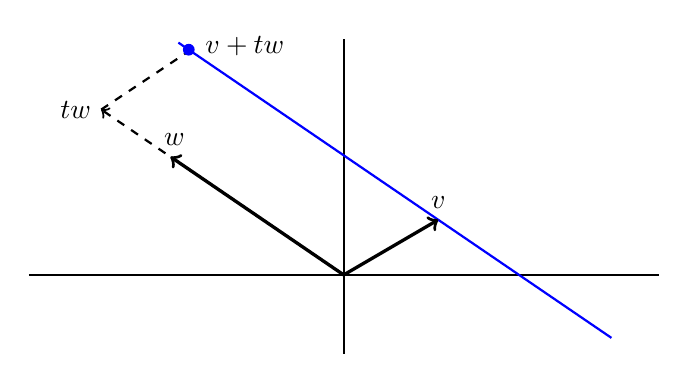
\begin{tikzpicture}
		\def\vx{1.2}
		\def\vy{0.7}
		\def\wx{-2.2}
		\def\wy{1.5}	
		\def\tw{1.4}					
		\draw[thick,-] (-4,0) -- (4,0);
		\draw[thick,-] (0,-1) -- (0,3);
		\draw[thick,blue,-] (\vx+1.5*\wx,\vy+1.5*\wy) -- (\vx-1*\wx,\vy-1*\wy);
		%\node[inner sep=1.5pt,fill,circle] at (\vx,\vy) {};
		\draw[very thick,->] (0,0) -- (\vx,\vy) node[above]{$v$};
		\draw[very thick,->] (0,0) -- (\wx,\wy) node[above]{\;$w$};
		\draw[dashed, thick,->] (0,0) -- (\tw*\wx,\tw*\wy) node[left]{$tw$};
		\draw[dashed,thick] (0,0) (\tw*\wx,\tw*\wy) -- (\vx+\tw*\wx,\vy+\tw*\wy+0.1);
		\node[inner sep=1.5pt,fill,circle,blue] at (\vx+\tw*\wx+0.04*\wx,\vy+\tw*\wy+0.04*\wy)  {};
		\node[right] at (\vx+\tw*\wx,\vy+\tw*\wy+0.1){$v+tw$};
		\end{tikzpicture}
	\end{center} 
\end{frame}



\begin{frame}
	Esta representación paramétrica también es útil para describir el conjunto de los puntos que se encuentran en el segmento de línea entre dos puntos dados. 
	\vskip .4cm\pause
	Sean $v$, $u$ dos puntos, entonces el segmento entre $v$ y $u$ consiste en todos los puntos
	\begin{equation*}
	S(t) = v + t(u-v)\quad  \text{con}\quad 0 \le t \le 1.
	\end{equation*}\pause
	Observar que 
	\begin{itemize}
		\item	en tiempo 0, $S(0) = v$,  y 
		\item  en tiempo 1, $S(1)= v + (u-v)= u$. 
	\end{itemize}
	
	\vskip .4cm\pause
	Como $t$ ``va'' de 0 a 1,  el móvil va de $v$ a $u$,  en linea recta.
\end{frame}



\begin{frame}
	Extendiendo a ambos lados el segmento, podemos describir la recta que pasa por $v$ y $u$ por la ecuación paramétrica
	\begin{equation*}
	S(t) = v + t(u-v)\quad  \text{con}\quad t \in \R.
	\end{equation*}
	\vskip .4cm
	\begin{figure}
		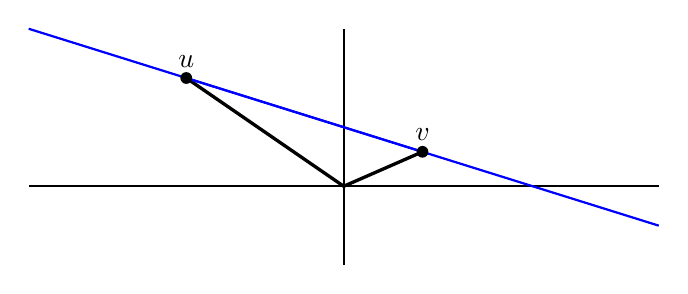
\begin{tikzpicture}
		\draw[thick,-] (-4,0) -- (4,0);
		\draw[thick,-] (0,-1) -- (0,2);
		\draw[blue,-] (-4,2) -- (4,-0.5);
		\draw[very thick,-] (0,0) -- (-4 + 8/4,2 -2.5/4) node[above]{$u$};
		\draw[very thick,-] (0,0) -- (-4 + 2.5*8/4,2 -2.5*2.5/4) node[above]{$v$};
		\draw[thick,blue,-] (-4 + 8/4,2 -2.5/4) -- (-4 + 2.5*8/4,2 -2.5*2.5/4);
		\draw[thick,blue,-] (-4,2) -- (4,-0.5);
		\node[inner sep=1.5pt,fill,circle,black] at (-4 + 8/4,2 -2.5/4) {};
		\node[inner sep=1.5pt,fill,circle,black] at (-4 + 2.5*8/4,2 -2.5*2.5/4)  {};
		\end{tikzpicture}
		\caption{La recta que pasa por $v$ y $u$.}
	\end{figure} 
	
	
\end{frame}



\begin{frame}
	\begin{ejemplo}
		Encontrar una representación paramétrica para la recta que contiene los puntos $(1, - 3, 1)$ y $(- 2,4,5)$.
	\end{ejemplo}	
	\begin{solucion} \pause Llamemos $v = (1, - 3, 1)$ y $u =(- 2,4,5)$.
		\vskip .4cm
		Entonces $u-v = (- 2,4,5) - (1,-3,1) = (-3,7,4)$ y la representación paramétrica de la recta que pasa por $u$ y $v$  es 
		\begin{equation*}
		X (t) = v + t(u-v) = (1, -3,1) + t (-3, 7, 4),\quad t\in \R.
		\end{equation*}
		\qed
	\end{solucion}
\end{frame}


\begin{frame}\frametitle{Ecuación implícita y ecuación paramétrica de la recta}
	Ahora discutiremos la relación entre una representación paramétrica y la ecuación implícita de una recta en el plano.
	\vskip .3cm \pause
	Sean $v, w \in \R^2$ con $w \not= 0$ y la recta descrita en forma paramétrica:
	\begin{equation*}
	X(t) =v +tw.
	\end{equation*}
		\vskip .3cm \pause
	Sea $v = (x_1,y_1)$, $w = (x_2,y_2)$. Todo punto de la recta es de la forma
	\begin{equation*}
	(x,y) =(x_1,y_1) +t(x_2,y_2) = (x_1+tx_2,y_1+ty_2),
	\end{equation*}\pause
	equivalentemente 
	\begin{equation*}
	x = x_1+tx_2, \qquad y = y_1+ty_2, \qquad
	\end{equation*}
	para $t \in \R$.
\end{frame}

\begin{frame}
	Es decir si la recta viene dada por 
		\begin{equation*}
	(x,y) =(x_1,y_1) +t(x_2,y_2),
	\end{equation*}
	tenemos que
	\begin{equation*}
	x = x_1+tx_2, \qquad y = y_1+ty_2. \qquad
	\end{equation*}
	
	Supongamos que $x_2 \not= 0$,  entonces
	 \begin{equation*}
	 x = x_1+tx_2, \qquad \Rightarrow \qquad t = \frac{x- x_1}{x_2}.
	 \end{equation*}
	 Reemplazando en la ecuación de $y$
	 \begin{equation*}
	 y = y_1+ty_2 =  y_1+\frac{x- x_1}{x_2}y_2 =  y_1+\frac{y_2}{x_2}x + \frac{-y_2}{x_2}y_2.
	 \end{equation*}

	 
\end{frame}

\begin{frame}
		 Es decir (multiplicando por $x_2$ y haciendo pasaje de término)
	\begin{equation*}
	{(-y_2)}x + x_2y =  x_2 y_1 {-y_2}y_2.
	\end{equation*}
	
	\vskip .6cm \pause
	
	 Si $x_2 =0$, como $w = (x_2,y_2) \not= 0$,  debe ser $y_2 \ne 0$ y se hace un razonamiento análogo.
	 	\vskip .3cm \vskip .3cm \pause
	 		
	 	\vskip 3cm 
\end{frame}



\begin{frame}
	\begin{ejemplo}
		Sean $v = (2, 1)$ y $w = (- 1, 5)$ y sea $X$ la recta que pasa por $v$  en la dirección $w$. Encontrar la ecuación  implícita de $X$.
		
	 \end{ejemplo}
\begin{solucion}\pause
{\footnotesize
La representación paramétrica de la recta que pasa por  $v$ en la dirección de $w$ es
\begin{equation*}
X(t)= (2,1)+ t(-1,5) = (2-t,1+5t).
\end{equation*}\pause
Es decir, si  miramos cada coordenada, 
\begin{equation}\label{eq-par-des-ej}
x = 2 - t, \qquad\quad y = 1 + 5t. \qquad\quad\tag{*}
\end{equation}



	Despejando $t$ de la primera ecuación obtenemos $t = 2-x$. 
	
	\vskip .3cm \pause
	
	Reemplazando este valor de $t$  en la segunda ecuación obtenemos
	\begin{equation*}
		y = 1 + 5t=1 + 5(2-x)t= y = 11- 5x,
	\end{equation*}\pause
	 luego
	\begin{equation}\label{eq-impl-rec-ej}
	5x + y = 11,\tag{**}
	\end{equation}
	que es la ecuación implícita de la recta.	\qed  }
\end{solucion}	


\end{frame}



\begin{frame}
	Recíprocamente, de la ecuación implícita podemos obtener la representación paramétrica. \pause
	
	\begin{ejemplo} Encontrar la representación paramétrica de la recta definida por 
		\begin{equation*}
		5x + 2y = 11. 
		\end{equation*}
	\end{ejemplo}
	\begin{solucion}\pause
		\vskip -.3cm
		\begin{equation*}
			5x + 2y = 11 \; \; \; \Rightarrow  \; \;\; 2y = 11 -5x   \;\;\; \Rightarrow   \;\;\; y =  - \frac{5}{2}x+\frac{11}{2}.
		\end{equation*}
		Remplazando $x$ por $t$ (sólo por notación) obtenemos que 
		\begin{equation*}
		Y(t) = (t,  - \frac{5}{2}t+\frac{11}{2})
		\end{equation*}
		es la representación paramétrica de la recta.\qed
	\end{solucion}	 
\end{frame}



\begin{frame}\frametitle{Planos en $\R^3$, interpretación geométrica}
		Comenzaremos, debido a que es más simple, con planos que  pasan por el origen,  como el de la siguiente figura.
		
		\vskip .3cm 
	\begin{figure}[h]
		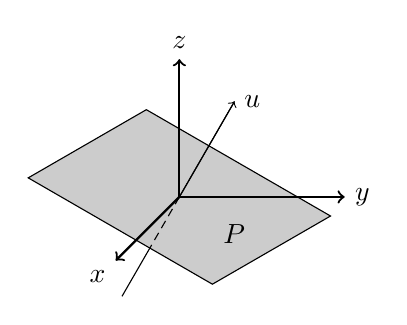
\begin{tikzpicture}[plane/.style={trapezium,draw,fill=black!20,trapezium left angle=60,trapezium right angle=120,minimum height=1.5cm},scale=0.7]
		\node (p)[plane,rotate=-30] at (0,0){.};
		\draw[rotate=-30] (p.center) edge ++(0,2cm) edge[densely dashed] (p.south) (p.south) edge ++(0,-1cm);
		\draw[->] (0,0,0) -- (2*0.5,2*0.866,0) node[right]{$u$};
		\draw[thick,->] (0,0,0) -- (3,0,0) node[right]{$y$};
		\draw[thick,->] (0,0,0) -- (0,2.5,0) node[above]{$z$};
		\draw[thick,->] (0,0,0) -- (0,0,3) node[anchor=north east]{$x$};
		\node [right] at (1.2,-0.1,1.5) {$P$};
		\end{tikzpicture}
		\caption{El plano $P$ y $u$, un vector  perpendicular al plano.}
	\end{figure} 
	

\end{frame}



\begin{frame}
		En  este caso,  es claro que el plano está determinado por un vector perpendicular al mismo.
		\vskip .3cm \pause
	Si $P$  es un plano que pasa por el origen y $u$ es un punto de $\R^3$, no nulo, tal que $u \perp P$,  entonces
	\begin{equation*}
	P = \{ v \in \R^3: \la v,u \ra=0 \}. 
	\end{equation*}
	\vskip 2cm
\end{frame}



\begin{frame}
		Sea ahora un  plano $P$ que no pasa por el origen y $v_0 \in P$.  
 \pause
	\begin{equation}\label{eq-p0-plano-1}
	P_0 = \{v-v_0: v \in P \}
	\end{equation} 
	es un plano que pasa por el origen. 
	\vskip .3cm \pause
	Luego,  si $u \perp P_0$,
	\begin{equation}\label{eq-p0-plano-2}
	P_0 = \{w: \la w,u \ra=0\}.
	\end{equation}
\vskip .3cm \pause

	De las ecuaciones (\ref{eq-p0-plano-1}) y  (\ref{eq-p0-plano-2}) deducimos que 
	\begin{equation*}
	v \in P \Leftrightarrow v-v_0 \in P_0 \Leftrightarrow \la v-v_0,u \ra=0.
	\end{equation*}
	\vskip .3cm \pause
	
	Es decir
	\begin{equation*}
	P = \{ v \in \R^3: \la v-v_0,u \ra=0 \}. 
	\end{equation*}
	Si $d = \la v_0,u \ra$,
	\begin{equation*}
	P = \{ v \in \R^3: \la v,u \ra=d \}. 
	\end{equation*}
\end{frame}



\begin{frame}\frametitle{Planos en $\R^3$. Definición}
		
	\begin{definicion} Sean $a,b, c,d \in \R$ tal que $(a,b,c) \ne (0,0,0)$ y sea 
		\begin{equation*}
		P = \{(x,y,z): ax +by +cz =d\}.
		\end{equation*}
		Entonces diremos que $P$  es  un \textit{plano con ecuación implícita}\index{plano en $\R^3$!ecuación implícita}  $ax +by +cz =d$ y  que $(a,b,c)$ es un \textit{vector normal al plano $P$.}
	\end{definicion} 
\vskip .4cm\pause
	 A esta forma de describir el plano también suele llamársela la \textit{ecuación normal del plano.}
	\vskip .4cm\pause

	Observar que la ecuación $ ax +by +cz =d$ no es más que la ecuación $\la(x,y,z),(a,b,c) \ra=d$. 	
	\vskip 1.2cm
\end{frame}



\begin{frame}
	\begin{ejemplo}
		El plano determinado por la ecuación
		\begin{equation*}
		2x - y 	+ 3z = 	5
		\end{equation*}
		es perpendicular al vector $(2, - 1, 3)$. 
		\vskip .4cm\pause
		¿Puntos del plano? Fijamos dos coordenadas y despejamos la tercera.
		\vskip .4cm\pause
		Por  ejemplo,  sea $x = 1$, $y = 1$ y despejamos $z$:
		\begin{equation*}
		3z 	= 5 - 2 + 1 = 4,
		\end{equation*}
		luego $z = \displaystyle\frac43$ y entonces
		\begin{equation*}
		(1,1,\frac43)
		\end{equation*}
		es un punto en el plano.
	\end{ejemplo}
\end{frame}



\begin{frame}
	Se dice que dos planos son \textit{paralelos} (en el 3-espacio) si sus vectores normales son paralelos,  es decir son proporcionales. 
	
	\vskip .8cm\pause
	
	Se dice que son \textit{perpendiculares} si sus vectores normales son perpendiculares. 
	
	\vskip .8cm\pause
	
	El \textit{ángulo entre dos planos} se define como el ángulo entre sus vectores normales.
	
	\vskip .4cm
	\vskip 2cm
	
\end{frame}



\begin{frame}\frametitle{Ecuación paramétrica del plano en $\R^3$}
  	
		\begin{definicion}
		Sean $v, w_1,w_2 \in \R^3$ tal que  $w_1$,$w_2$ no  nulos y tal que $w_2$ no sea un múltiplo de $w_1$. Sea 
		\begin{equation*}
		P = \{v + sw_1 + tw_2: s,t \in \R\}. 
		\end{equation*}
		Diremos entonces que  \textit{$P$ es el  plano a través de $v$ paralelo a los vectores $w_1$ y $w_2$.}\index{plano en $\R^3$!ecuación paramétrica} 
	\end{definicion}
\vskip .4cm
	


\end{frame}

\begin{frame}
	Si 
	\begin{equation*}
	P = \{v + sw_1 + tw_2: s,t \in \R\},
	\end{equation*}
	entonces el vector $v$ pertenece al plano y el plano 
	\begin{equation*}
	P_0 = \{sw_1 + tw_2: s,t \in \R\}
	\end{equation*}
	es el plano que pasa por el origen y paralelo a $P$. 
\end{frame}

\begin{frame}
	
	Si $P = \{(x,y,z): ax +by +cz =d\}$ con $a\ne 0$.
	\vskip .4cm
	Podemos poner $x$ en función de  $y$, $z$ y los datos. Así obtenemos una ecuación paramétrica de $P$. 
	\vskip .4cm\pause
	Se puede hacer de forma análoga cuando $b\ne 0$ o $c \ne 0$. 
	
		\vskip .4cm\pause

\end{frame}

\begin{frame}
		\begin{ejemplo}
		Sea $P = \{(x,y,z): x -2y +z =1\}$. 
		\vskip .4cm
		Como  $x -2y +z =1$ sii  $x = 2y-z +1$, tenemos que
		\begin{equation*}
		P = \{(2y-z +1,y,z): y,z \in \R\},
		\end{equation*}\pause
		o,  escrito de una forma más estándar,
		\begin{equation*}
		P = \{(2s-t +1,s,t): s,t \in \R\}. 
		\end{equation*}
		
		También podemos escribir
		\begin{equation*}
		P = \{(1,0,0) + s(2,1,0) + t(-1,0,1): s,t \in \R\}. 
		\end{equation*}
		\qed
		
	\end{ejemplo}
\end{frame}





\begin{frame}
	¿Cómo obtenemos la ecuación normal del plano?
	\vskip .4cm\vskip .4cm\pause
	Si encontramos $u \ne 0$ tal que $\la u,w_1 \ra =0$ y $\la u,w_2 \ra =0$, entonces $ \la  sw_1 + tw_2, u \ra =0$ para  $s,t$ arbitrarios y 
	\begin{equation*}
	P_0 = \{(x,y,z): \la (x,y,z),u \ra =0\}. 
	\end{equation*}\pause	\vskip .1cm
	Sea $d = \la v, u \ra$, entonces $\la v + sw_1 + tw_2, u\ra = \la v , u\ra =d$, para $s,t$ arbitrarios. Es decir
	\begin{equation*}
	P = \{(x,y,z): \la (x,y,z),u \ra =d\}. 
	\end{equation*}
\end{frame}



\begin{frame}
		\begin{ejemplo}
		Sea $P = \{ (1,1,0) + s(-1,0,-1) + t(0,1,-2): s,t \in \R\}$. Encontrar la ecuación implicita de $P$.
		\end{ejemplo}
		\begin{solucion}\pause
			Sea $u= (a,b,c)$,  entonces 
			\begin{align*}
			\la u,(-1,0,-1) \ra = 0 \quad &\Leftrightarrow \quad -a -c=0 \quad\Leftrightarrow   \quad a = -c, \\
			\la u,(0,1,-2) \ra = 0 \quad &\Leftrightarrow \quad b -2c=0 \quad\,\Leftrightarrow \quad b=2c.
			\end{align*} 
			Luego $u=(-c,2c,c)$. Si, por ejemplo, $c=1$, $\Rightarrow$ $u=(-1,2,1)$, luego:
			\begin{equation*}
			P_0 = \{(x,y,z): -x+2y+z =0\}. 
			\end{equation*}
			Como $\la (1,1,0),(-1,2,1) \ra = 1 $, obtenemos
			\begin{align*}
			P &= \{(x,y,z): \la (x,y,z),(-1,2,1) \ra =1\} \\
			&= \{(x,y,z): -x+2y+z =1\}.
			\end{align*}
			\qed
		\end{solucion}
		

\end{frame}





\end{document}

